\documentclass[10pt,xcolor={usenames,dvipsnames,table}]{beamer}
\usepackage{tri_preamble}

%----------------------------------------------------------------------------------------
%	TITLE PAGE
%----------------------------------------------------------------------------------------

\title{Structure Learning} % The short title appears at the bottom of every slide, the full title is only on the title page

\author{Tri Nguyen} % Your name

\institute[OSU] % Your institution as it will appear on the bottom of every slide, may be shorthand to save space
{
    Internal Presentation  \\
Oregon State University  % Your institution for the title page
% \medskip
% \textit{nguyetr9@oregonstate.edu \endgraf } % Your email address
% }
}
\date{\today} % Date, can be changed to a custom date


\makeatletter
\makeatother


\begin{document}

\frame{\titlepage}

\begin{frame}
    \frametitle{Main Reference}
    \fullcite{zheng2018dags}
\end{frame}


\begin{frame}
\frametitle{Some Definitions}
\begin{itemize}
    \item \textbf{Directed Acyclic Graph (DAG)}. A graph $G$ is a DAG if it is directed and there is no cycle. 
        \begin{itemize}
            \item \textbf{d-separation}. 3 vertices is called $A \indep_{G} B | C$ if they form either a chain, fork, or collider in $G$ (in a particular order).
                \begin{figure}
                    \centering
                    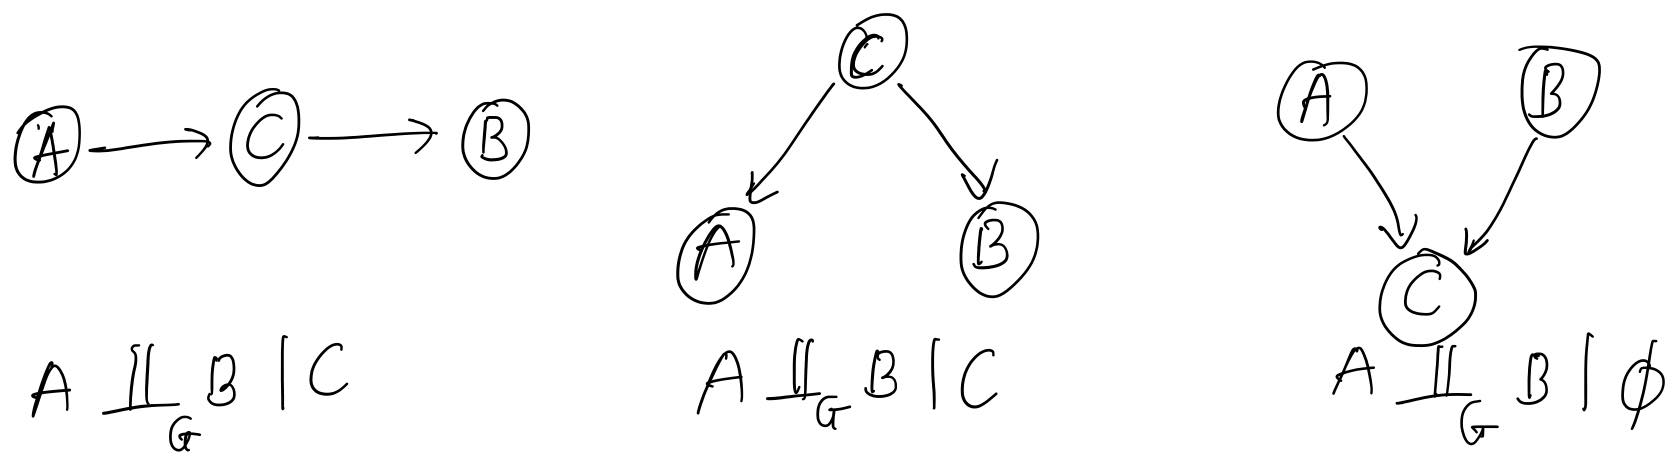
\includegraphics[width=0.7\textwidth]{figures/chain_folk_collider.jpg}
                \end{figure}
        \end{itemize}
    \item \textbf{Markov assumption}. A joint probability $P$ is Markov compatible to a DAG $G$ iff
        \[
        P(X_1, \ldots , X_p) = \prod_{i} P(X_i | \text{pa}_i)
        \] 
    \begin{itemize}
    \item $P$ is Markov compatible to  $G$ iff
        \[
        \bm{A} \indep_{G} \bm{B} \mid \bm{C} \Rightarrow \bm{A} \indep_{P} \bm{B} \mid \bm{C}
        \] 
    \end{itemize}
\end{itemize}
\end{frame}

\begin{frame}
\frametitle{Some Definitions}
\begin{itemize}
    \item \textbf{Minimality} (informal). $G$ is the ``smallest graph'' that is compatible with $P$.
\item \textbf{Faithfulness assumption}. $P$ is faithful to  a DAG $G$ iff
     \[
        \bm{A} \indep_{P} \bm{B} \mid \bm{C} \Rightarrow \bm{A} \indep_{G} \bm{B} \mid \bm{C} 
    \] 
    \begin{itemize}
        \item Faithfulness and Markov assumption leads to minimality.
    \end{itemize}
    \item \textbf{Markov equivalence}. Set of all minimal DAG $G$ that are Markov compatible to $P$.
\begin{figure}
    \centering
    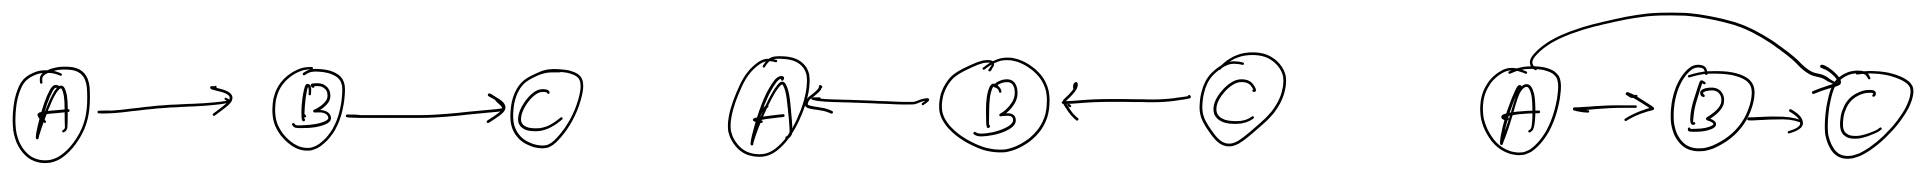
\includegraphics[width=0.7\textwidth]{figures/equivalence_class.jpg}
    \caption*{$P(X_1, X_2, X_3) = P(X_1|X_2) P(X_3|X_2) P(X_2)$. }
\end{figure}
\end{itemize}
\end{frame}

\begin{frame}
    \frametitle{Problem}
    \begin{block}{Structure Identification}
        Given $n$ i.i.d data $\bm{X} \in \mathbb{R}^{n \times p}$ that are generated from some $P(X_1, \ldots , X_p)$, can we identify a minimal DAG $G$ up to Markov equivalence?
    \end{block}
\begin{figure}
    \centering
    \begin{subfigure}{0.45\textwidth}
    \resizebox{0.8\textwidth}{!} {
    \begin{tikzpicture}
        \node[latent](X1){$X_1$};
        \node[latent, right=of X1](X2){$X_2$};
        \node[latent, right=of X2](X3){$X_3$};
        \draw[->] (X1) -- (X2);
        \draw[->] (X2) -- (X3);
    \end{tikzpicture}
}
\subcaption*{ $G_1$ }
    \label{fig:markov_equiv_1}
    \end{subfigure}
    \begin{subfigure}{0.45\textwidth}
    \resizebox{0.8\textwidth}{!}{
    \begin{tikzpicture}
        \node[latent](X1){$X_1$};
        \node[latent, right=of X1](X2){$X_2$};
        \node[latent, right=of X2](X3){$X_3$};
        \draw[->] (X1) -- (X2);
        \draw[->] (X2) -- (X3);
        \draw[->] (X1) to [out=30,in=150] (X3);
    \end{tikzpicture}
}
    \subcaption*{ $G_2$ }
    \label{fig:markov_equiv_2}
    \end{subfigure}
    \caption*{If the ground truth $P(X_1, X_2, X_3) = P(X_1|X_2)P(X_3|X_2)P(X_2)$, can we recover $G_1$ (or its equivalence) from observational data?}
\end{figure}

    \note{The name structure Identification because we don't ``care'' about coefficient, or maybe too hard to get them.

        Clearly, graph has no weights.
    }
\end{frame}

\begin{frame}
    \frametitle{Constraint-based Approach: The PC-Algorithm}
    \begin{figure}
        \centering
        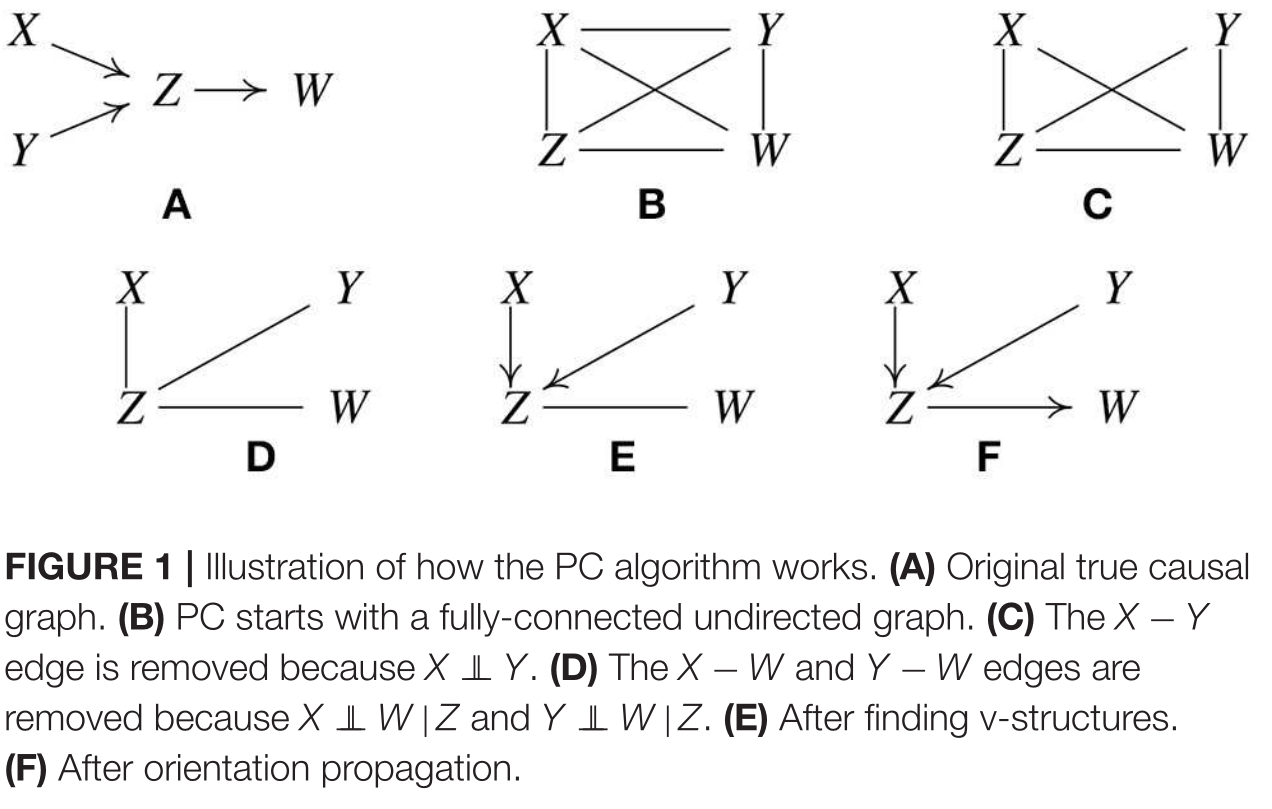
\includegraphics[width=0.8\textwidth]{figures/pc.png}
        \caption*{\citep{glymour2019review}}
    \end{figure}
    \begin{itemize}
        \item Step 1: Identify the skeleton (A-D)
        \item Step 2: Identify v-structures and orient them (E)
        \item Step 3: Identify qualifying edges that are incident on collider (F)
    \end{itemize}
\end{frame}

\begin{frame}
    \frametitle{Structural Equation Model}
    \begin{itemize}
        \item Another representation named Structural Equation Model (SEM) is used to model relationship among variables.
    \[
    X_i = f(\text{Pa}_i, z_i),
    \] 
    where $z_i$ is independent to all variables in $\text{Pa}_i$, and all $z_i$s are mutually independent.
    \item One popular consideration is linear  function, and some/all of $z_i$ follow Gaussian distribution \citep{loh2014high,van2013ell_}.

    \item In \citep{zheng2018dags}, $f$ is assumed as
        \[
        X_i = w_i^{\T} \text{Pa}_i + z_i
        \] 
        Then a DAG $G$ can be represented by an adjacency matrix  $\bm{W} \in \mathbb{R}^{p \times p}$ such that
        \begin{itemize}
            \item $w_{ij} \neq 0 \Leftrightarrow (i \rightarrow j)$ is an edge in $G$. Denote such constructed graph $G(\bm{W})$.
            \item  $X_i = \bm{W}(:,i)^{\T}X + z_i$.
        \end{itemize}

    \end{itemize}


\end{frame}
\begin{frame}
    \frametitle{Score-based Approach}
    \begin{figure}
        \centering
        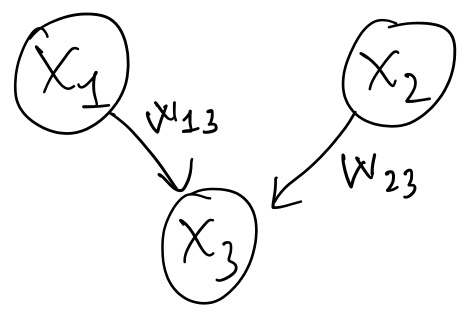
\includegraphics[width=0.3\textwidth]{figures/graph.jpg}
    \end{figure}
    A general formulation,
    \begin{alignat*}{2}
        & \maximize_{G} \quad && s(\bm{W}) \\
        & \text{\rm subject to} && G(\bm{W}) \text{ is a DAG} 
    \end{alignat*}

    \begin{itemize}
        \item Many score function $s(\cdot)$ have been developed that guarantee identifiability of $G$, such as Bayesian information criterion (BIC).

            For example,
        $\norm{\bm{X} - \bm{X}\bm{W}}_{\rm F}^2 + \lambda r(\bm{W})$ is used in case of Gaussian linear structural model \citep{van2013ell_}.
        \item However, dealing with the constraint is difficult. The problem is NP-hard \citep{chickering2004large}.
        \item A pioneer work is greedy equivalence search (GES) \citep{chickering2002optimal}. 
            % It searches over a ``sparse search space'' and greedily pick a local best candidate according to some scoring function (Bayesian information criterion).
    \end{itemize}
\end{frame}

\begin{frame}
    \frametitle{Score-based Approach}
    \begin{equation*}
    \begin{aligned}
        &\min_{\bm{W} \in \mathbb{R}^{d \times d}}  & & s(\bm{W}) \\
        &\text{subject to} && G(\bm{W}) \in \texttt{DAG}
    \end{aligned}
    \quad 
    \Leftrightarrow
    \quad 
    \begin{aligned}
        &\min_{\bm{W} \in \mathbb{R}^{d \times d}}  & & s(\bm{W}) \\
        &\text{subject to} && h(\bm{W}) = 0
    \end{aligned}
    \end{equation*}
    where we wish $h$ to be
    \begin{itemize}
        \item $h(\bm{W}) = 0$ if and only if $G(\bm{W})$ is acyclic.
        \item $h(\bm{W}) = 0$ measures the ``DAG-ness'' of the graph.
        \item $h(\bm{W})$ is smooth.
        \item $h(\bm{W})$ and its derivatives are easy to compute.
    \end{itemize}
\end{frame}

\begin{frame}
    \frametitle{Binary Case}
    \begin{proposition}[Infinite series]
        Suppose $\bm{B} \in \set{0,1}^{p \times p}$ and $\abs{\lambda_{\max}(\bm{B})} < 1$. Then $G(\bm{B})$ is a DAG if and only if 
        \[
        \text{tr}(\mathbf{I} - \bm{B})^{-1} = p.
        \] 
    \end{proposition}
    \begin{proof}
        \begin{itemize}
            \item Number of length-$2$ paths from $i$ to $j$ is  $\sum^{p}_{t=1} B(i, t) B(t, j) = \bm{B}^{2}(i, j)$.
            \item Number of length-$k$ paths from $i$ to  $j$ is  $\bm{B}^{k}(i, j)$.
            \item Number of closed length-$k$ paths from $i$ to $i$ is $\bm{B}^{k}(i, i)$.
            \item Number of closed length-$k$ paths is  $\text{tr} (\bm{B}^{k})$.
            \item A graph is acyclic if and only if 
                $ \sum^{\infty}_{k=1} \text{tr}(\bm{B}^{k}) = 0$ 
        \end{itemize}

    \end{proof}
\end{frame}
\begin{frame}
    For any square matrix $\bm{B}$,
    \begin{align*}
        (\bm{I} - \bm{B})^{-1} 
        &= \bm{I} + (\bm{I} - \bm{B})^{-1} \bm{B} \\
        &= \bm{I} + (\bm{I} + (\bm{I}-\bm{B})^{-1}\bm{B}) \bm{B} \\
        &= \ldots  \\
        &= \bm{I}+ \bm{B} + \bm{B}^{2} + \ldots 
    \end{align*} 
    \[
    \text{tr}\left((\bm{I} - \bm{B})^{-1}\right) = \text{tr}(\bm{I}) + \sum^{\infty}_{k=1} \text{tr}(\bm{B}^{k}) = p
    \] 

%     Note that 
%     \[
%     \abs{\lambda_{\max}(\bm{B})} < 1, \bm{B}^{k} \xrightarrow{k \to \infty} \textbf{0}
% \]
    % Therefore
    % \[
    % (\bm{I} - \bm{B})^{-1} = \sum^{\infty}_{k=0} \bm{B}^{k} \text{ is well defined}
    % \] 
\end{frame}

\begin{frame}
    \frametitle{A Better Formula}

    \begin{proposition}
        A binary matrix $\bm{B} \in \set{0, 1}^{d \times d}$ is a DAG if and only if 
        \[
        \text{tr} (e^{\bm{B}}) = d.
        \] 
        where 
\[
e^{\bm{B}} := \sum^{\infty}_{k=0} \dfrac{1}{k!} \bm{B}^{k}
\] 

    \end{proposition}
    \begin{block}{Remark}
        \begin{itemize}
            \item $e^{\bm{B}}$ is always well-defined for all square matrix $\bm{B}$.
            \item The equivalence of having no cyclic path and $\text{tr}(\bm{B}^{k}) = 0$ for all $k$ only hold if $\bm{B}>0$.
        \end{itemize}
    \end{block}
\end{frame}

\begin{frame}
    \frametitle{Arbitrary Weight Matrix $\bm{B}$}
    \begin{theorem}
        For $\bm{W} \in \mathbb{R}^{p\times  p}$, $G(\bm{W})$ is a DAG iff 
        \[
        h(\bm{W}) := \text{tr} \left( e^{\bm{W}*\bm{W}} \right) - d = 0
        \] 
    \end{theorem}
    \begin{block}{Remark}
        \begin{itemize}
            \item Gradient of $h$ is $\nabla h(\bm{W}) = (e^{\bm{W} * \bm{W}})^{\T} * 2\bm{W}$.
            \item Evaluating $e^{\bm{W}}$ costs $O(p^{3})$ \citep{al2010new}.
        \end{itemize}
    \end{block}
    To this end,
    \begin{alignat*}{2}
        & \minimize_{W} \quad && \dfrac{1}{2n}\norm{\bm{X} - \bm{W}\bm{X}}_{\rm F}^2 + \lambda \norm{\bm{W}}_1\\
        & \text{subject to} && \text{tr}(e^{\bm{W} * \bm{W}}) = d
    \end{alignat*}
    and \citep{zheng2018dags} solved it using augmented Lagrange method.
\end{frame}

\begin{frame}
    \frametitle{Experiment Result}
    Baseline
    \begin{itemize}
        \item PC-algorithm is excluded since GES and NOTEARS outperforms it significantly.
        \item A fast version of GES named FGS is used \citep{ramsey2017million}
    \end{itemize}
    Data
    \begin{itemize}
        \item Generate a random graph $G$ by Erdös-Rényi (ER) or scale-free (SF) model.
        \item Generate uniform $\bm{W}$ respect to graph $G$.
        \item Sample noise according to Gaussian, Exponential, and Gumble distribution.
        \item Finally, generate data $\bm{X} \in \mathbb{R}^{n \times p}$ for $p \in \set{10, 20, 50, 100}$, and $n \in \set{20, 10000}$.
    \end{itemize}
\end{frame}

\begin{frame}
    \frametitle{Experiment Result}
    \begin{figure}
        \centering
        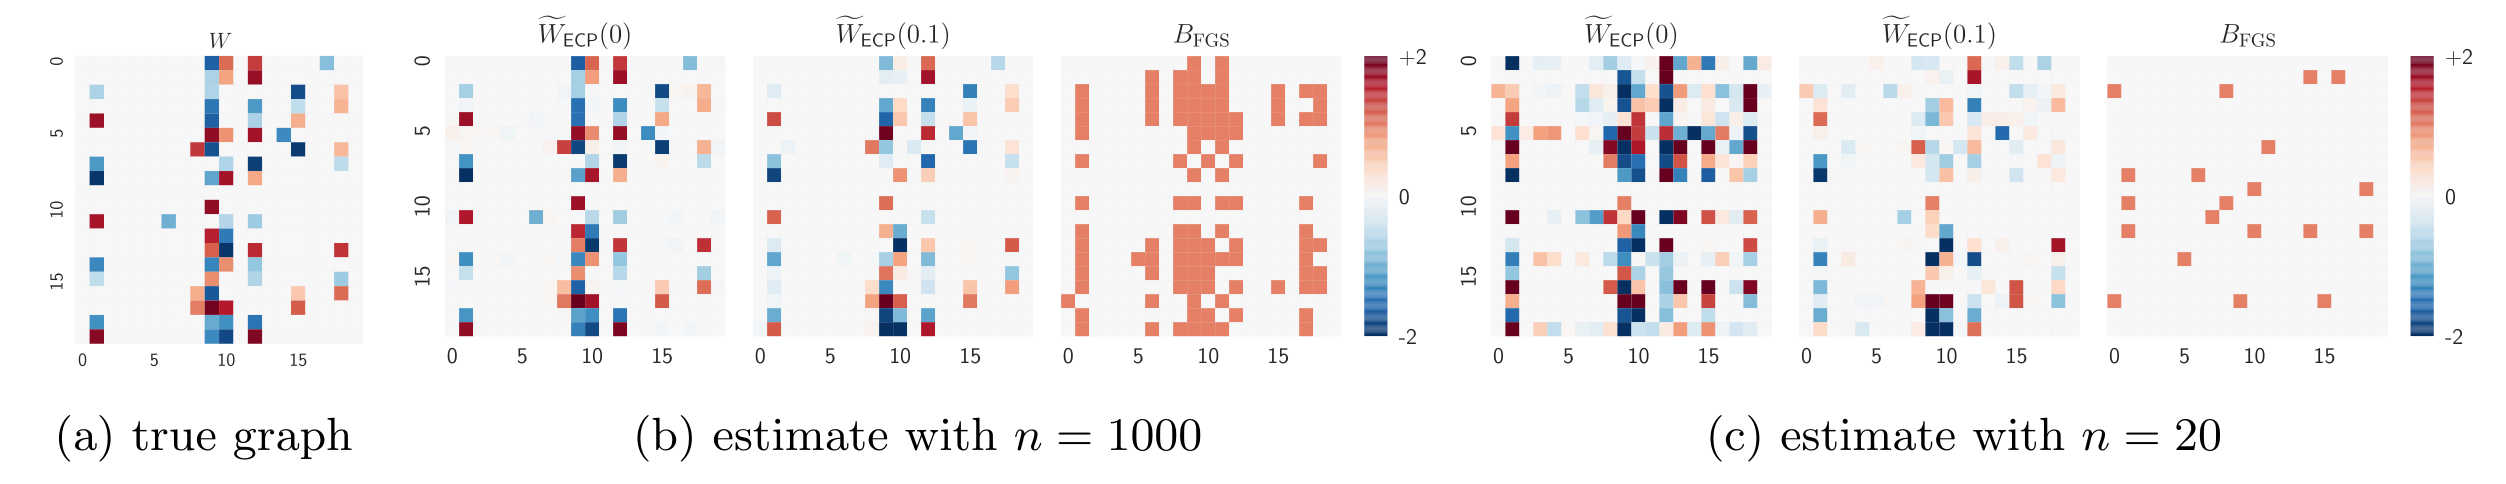
\includegraphics[width=\textwidth]{figures/result1.png}
    \end{figure}
\end{frame}

\begin{frame}
    \frametitle{Experiment Result}
    \begin{figure}
        \centering
        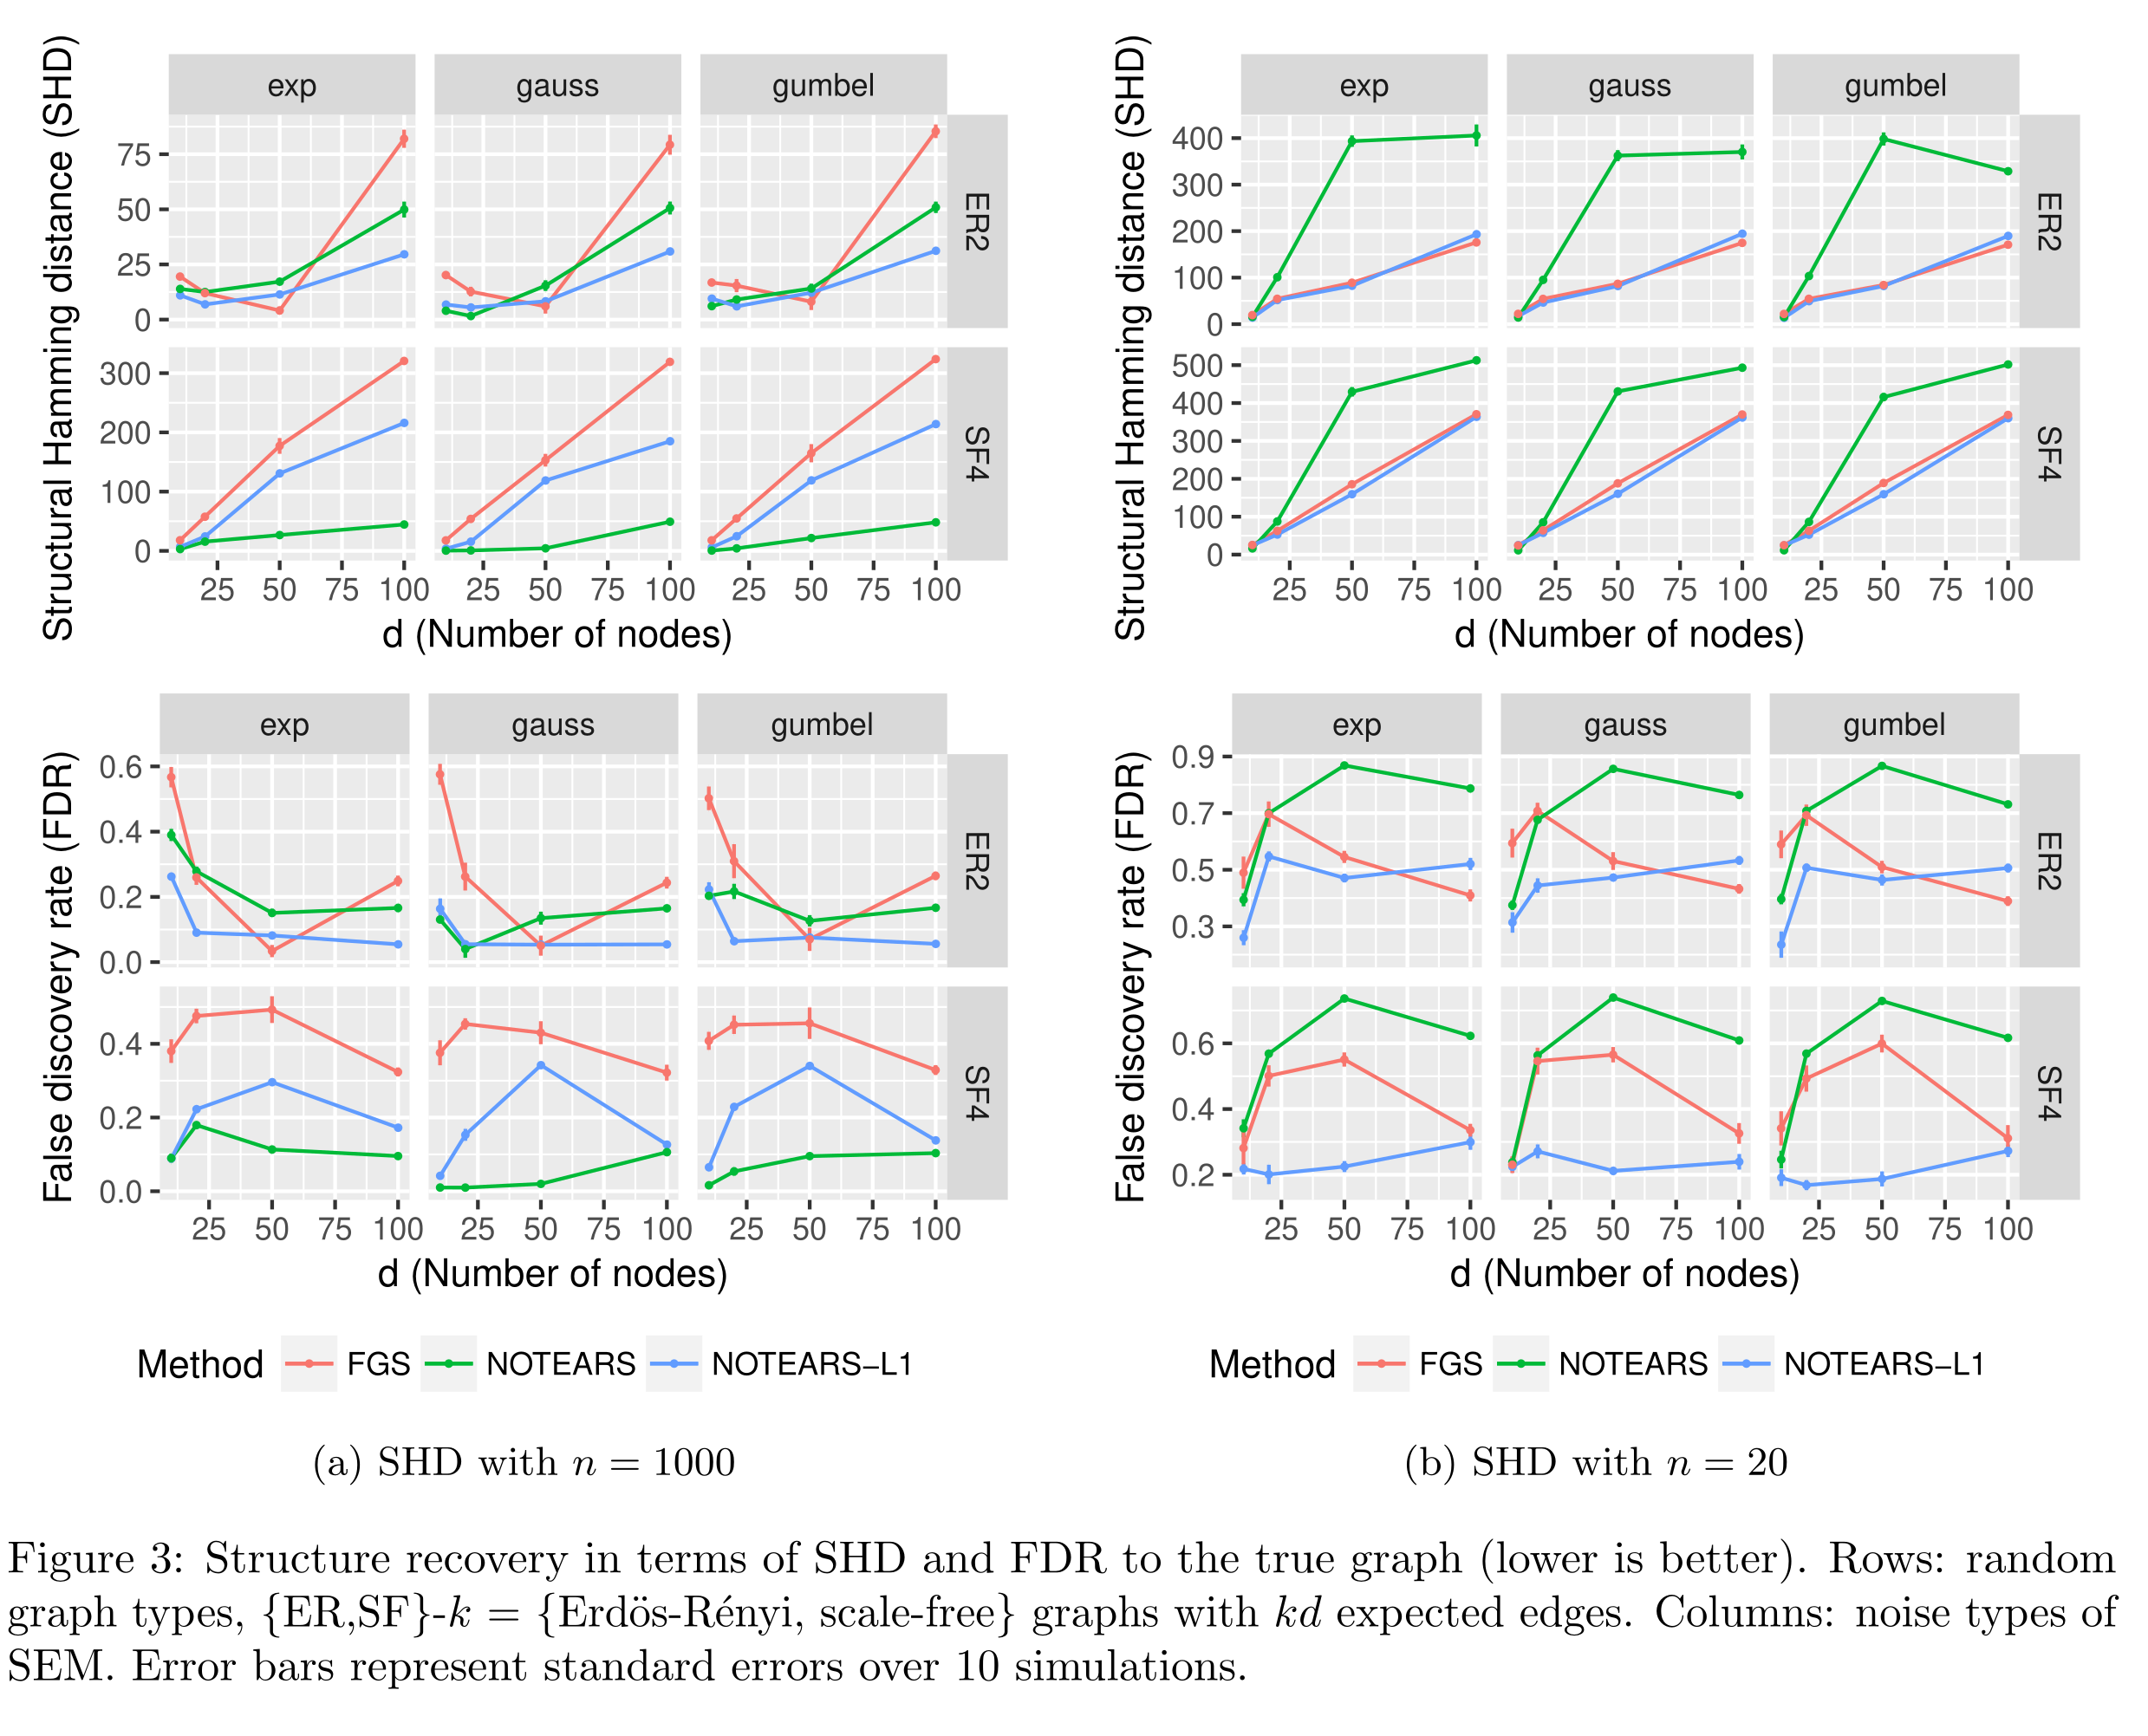
\includegraphics[width=\textwidth]{figures/result2.png}
    \end{figure}
\end{frame}

\appendix
\begin{frame}[allowframebreaks]
    \frametitle{Reference}
    \printbibliography
\end{frame}

\begin{frame}
    \frametitle{Bayesian Network}
    A Bayesian network is a tuple of 2 components: $U, G=<V, E>$.
     \begin{itemize}
        \item $U={X_1, \ldots , X_p}$: set of random variables.
        \item $G$ is a directed acyclic graph, where vertex $V_i$ represents $X_i$. 
    \end{itemize}
    Altogether, a BN defines a joint distribution $P(X_1, \ldots , X_p)$ as
    \[
    P(X_1, \ldots , X_p) = \prod_{i}^{p} P(X_i| \text{pa}_i)
    \] 

    Assume $X$ is satisfied
    \[
    X_i = w_i^{\T} \text{pa}_i + z_i
    \] 
    where $z_i$ is some noise. All $z_i$ are mutually independent.

    Now, given dataset, how do we identify graph $G$ (or find $W$)?
\end{frame}
%
% \begin{frame}
%     \frametitle{Approaches}
%     A natural perspective
% \begin{alignat*}{2}
%     & \maximize_{G} \quad && Q(G) \\
%     & \text{subject to} && G \in \mathcal{D}
% \end{alignat*}
% where $\mathcal{D} =\set{\text{all DAG graphs of $p$ vertices}}$, and
% \begin{itemize}
%     \item $Q(G)$ is some score function to justify how $G$ fits data.
%     \item NP-hard problem \citep{chickering2004large} due to combinatorial and nonconvex nature of the problem.
% \end{itemize}
% Two main approaches:
%     \begin{itemize}
%         \item Constraint-based method (PC algorithm \citep{spirtes2000causation})
%            \begin{itemize}
%                \item Utilize independence tests
%                \item Identifiability results are guaranteed under faithfulness assumption.
%            \end{itemize}
%         \item Score-based methods
%     \end{itemize}
% \end{frame}
%
% \begin{frame}
%     \frametitle{The PC-Algorithm}
%     \begin{figure}
%         \centering
%         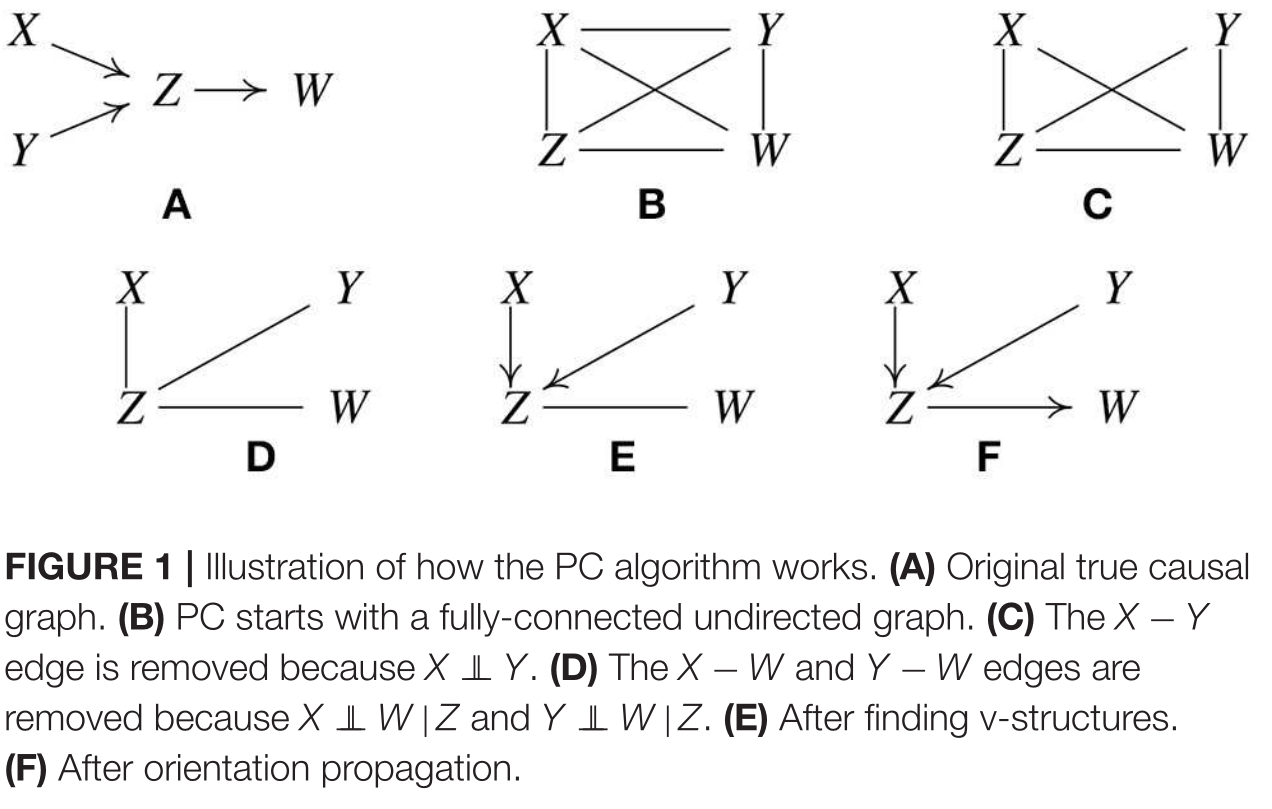
\includegraphics[width=0.8\textwidth]{figures/pc.png}
%     \end{figure}
%     \begin{itemize}
%         \item Identify the skeleton (A-D)
%         \item Identify immoralities and orient them (E)
%         \item Identify qualifying edges that are incident on collider (F)
%     \end{itemize}
% \end{frame}
%
% \begin{frame}
%     \frametitle{Score-based Approach}
% \begin{alignat*}{2}
%     & \maximize_{G} \quad && Q(G) \\
%     & \text{subject to} && G \in \mathcal{D}
% \end{alignat*}
%     \begin{itemize}
%         \item There are several scores function that have little prior knowledge (class of conditional distributions), such as BIC, BD, \ldots 
%         \item Other works restrict distribution class. For example, NOTEAR \cite{} assume a linear case 
%         \item Other includes BD, BDu, \ldots 
%     \end{itemize}
% \end{frame}
% \begin{frame}
%     \frametitle{Scores}
%     % Assume the joint probability $P$ is parameterized by set of  $\theta_{X_i}, i=1,\ldots ,p$.
%     \begin{itemize}
%         % \item By Markov assumption,
%         %     \[
%         %     P(\bm{X} | G, \Theta) = \prod_{i=1}^{p} P(X_i | \text{pa}_{X_i}, \theta_{X_i})
%         %     \] 
%         \item For learning $G$, $P(G|D) \propto  P(D|G) P(G)$ , and under several assumptions, several closed-form expression has been derived (BIC, BD, \ldots )
%         \item For example, if $X_i \sim \mathcal{N}(\mu_i, \sigma_i)$ and follows a linear model, then 
%     \end{itemize}
%     
% \end{frame}
%
% \begin{frame}
% \frametitle{Structural Equation Model}
% \begin{itemize}
%     \item A graph $G$ is directed acyclic graph (DAG) if it is directed and there is no cyclic. 
%     \item Given a DAG $G$ and a joint distribution  $P(X_1, \ldots , X_p)$. Graph $G$ is called \textbf{Markov relative} to  $G$ if 
%                 \[
%         P(X_1, \ldots , X_p) = \prod_{i} P(X_i | \text{pa}_i)
%                 \] 
%     \item $P$ is Markov relative to  $G$ iff
%         \[
%         A \indep_{G} B \mid C \Rightarrow A \indep B |\mid C
%         \] 
%         where $\indep_{G}$ denotes d-separation property.
%     \item Consider a class $\mathcal{D}$ of directed acyclic graph $G=\langle V, E \rangle$ where $V=\set{X_1, \ldots , X_p}$.
%         A joint pdf $P(X_1, \ldots , X_p)$ is called \textbf{Markov relative} to $G \in \mathcal{D}$ if
%         \[
%         P(X_1, \ldots , X_p) = \prod_{i} P(X_i | \text{pa}_i)
%         \] 
%         where $\text{pa}_i$ is set of parent of $X_i$ in $G$ [x]
%     \item 
%
%     \item \textbf{Structural equation models (SEM)} is a set of $p$ equations that describes relationship between  $p$ RVs, i.e., 
% \[
% X_i = f_i(\text{pa}_i, \epsilon_i), \text{ for } i=1, \ldots , p
% \]
% and $\text{pa}_i$ is a subset of $\set{X_1, \ldots , X_p}$ that directly determine the value of $X_i$, and $\epsilon_i$s are mutually independent, and also independent with $\text{pa}_i$ [x].
%
% \item The ``structure'' part of a SEM can be shown using a directed acyclic graph.
%
% \item Problem: Given $n$ i.i.d data points $\bm{X} \in \mathbb{R}^{n\times  p}$, can we recover $f_i$?
% \item A linear SEM is a SEM with all $f_i$ being linear functions, i.e.,
%      \[
%     X_i = \sum_{X_j \in \text{pa}_i} w_j X_j + \epsilon_i
%     \] 
% \end{itemize}
%
% \end{frame}
%
%
% \begin{frame}
% \frametitle{Structural Equation Model (SEM)}
%
% \begin{definition}[Markov constraints]
% Let a graph $G=\langle V, E \rangle$ be directed acyclic graph (DAG). Markov constraints are set of independence relations defined by $G$.
% \end{definition}
% \begin{definition}[Markov equivalent]
% Two DAGs are Markov equivalent if they have the same Markov constraints.
% \end{definition}
%
% \begin{figure}
%     \centering
%     \begin{subfigure}{0.3\textwidth}
%     \resizebox{0.8\textwidth}{!} {
%     \begin{tikzpicture}
%         \node[latent](A){$A$};
%         \node[latent, right=of A](B){$B$};
%         \node[latent, right=of B](C){$C$};
%
%         \edge{A}{B};
%         \edge{B}{C};
%     \end{tikzpicture}}
%     \subcaption{ }
%     \label{fig:markov_equiv_1}
%     \end{subfigure}
%     \begin{subfigure}{0.3\textwidth}
%     \resizebox{0.8\textwidth}{!}{
%     \begin{tikzpicture}
%         \node[latent](A){$A$};
%         \node[latent, right=of A](B){$B$};
%         \node[latent, right=of B](C){$C$};
%
%         \edge{B}{A};
%         \edge{C}{B};
%     \end{tikzpicture}}
%     \subcaption{ }
%     \label{fig:markov_equiv_2}
%     \end{subfigure}
%     \begin{subfigure}{0.3\textwidth}
%     \resizebox{0.8\textwidth}{!}{
%     \begin{tikzpicture}
%         \node[latent](A){$A$};
%         \node[latent, right=of A](B){$B$};
%         \node[latent, right=of B](C){$C$};
%
%         \edge{A}{B};
%         \edge{C}{B};
%     \end{tikzpicture}}
%     \subcaption{ }
%     \label{fig:markov_equiv_2}
%     \end{subfigure}
%     \caption{(a) and (b) are Markov equivalent, while (c) are not. Both (a) and (b) have only one Markov constraint $A \indep C | B$, while in (c), it is $A \indep C$.}
% \end{figure}
% {\red what is $A \rightarrow B$?}
% \begin{block}{Goal}
%     Determine $G$ up to Markov equivalent ambiguity.
% \end{block}
% \end{frame}
%
% \begin{frame}
% \frametitle{Another example}
% \begin{figure}
%     \centering
%     \begin{subfigure}{0.2\textwidth}
%     \resizebox{0.8\textwidth}{!} {
%     \begin{tikzpicture}
%         \node[latent](A){$A$};
%         \node[latent, below=of A](B){$B$};
%         \node[latent, below=of B, xshift=-1.5cm](C){$C$};
%         \node[latent, below=of B,xshift=+1.5cm](D){$D$};
%
%         \edge{A}{B};
%         \edge{B}{C,D};
%         \edge{C}{D};
%     \end{tikzpicture}}
%     \subcaption{ }
%     \label{fig:markov_equiv_1}
%     \end{subfigure}
%     \begin{subfigure}{0.2\textwidth}
%     \resizebox{0.8\textwidth}{!}{
%     \begin{tikzpicture}
%         \node[latent](A){$A$};
%         \node[latent, below=of A](B){$B$};
%         \node[latent, below=of B, xshift=-1.5cm](C){$C$};
%         \node[latent, below=of B,xshift=+1.5cm](D){$D$};
%
%         \edge{B}{A};
%         \edge{B}{C,D};
%         \edge{C}{D};
%     \end{tikzpicture}}
%     \subcaption{ }
%     \label{fig:markov_equiv_2}
%     \end{subfigure}
%     \begin{subfigure}{0.2\textwidth}
%     \resizebox{0.8\textwidth}{!}{
%     \begin{tikzpicture}
%         \node[latent](A){$A$};
%         \node[latent, below=of A](B){$B$};
%         \node[latent, below=of B, xshift=-1.5cm](C){$C$};
%         \node[latent, below=of B,xshift=+1.5cm](D){$D$};
%
%         \edge{A,C}{B};
%         \edge{B}{D};
%         \edge{C}{D};
%     \end{tikzpicture}}
%     \subcaption{ }
%     \label{fig:markov_equiv_2}
%     \end{subfigure}
%     \caption{(a) and (b) are Markov equivalent, while (c) are not.}
% \end{figure}
% \begin{definition}[Skeleton]
%     A undirected induced from DAG $G$ is skeleton of  $G$.
% \end{definition}
% \begin{definition}[Immorality]
%     A subgraph of 3 nodes $X, Y, Z$ induced for a DAG $G$  is called immorality if $X \rightarrow Z$,  $Y \rightarrow Z$ and $X, Y$ are non-adjacent.
% \end{definition}
%     
% \begin{theorem}[A well known result]
%     Two DAGs are equivalent if they have the same skeleton and same set of immoralities.
% \end{theorem}
% \end{frame}
%
% \subsection{Constraint-based Approach}%
% \begin{frame}
% \frametitle{Constraint-based Approach: the PC Algorithm}
% some demo of the method
% \end{frame}
%
% \begin{frame}
% \frametitle{Pros and Cons}
% \begin{itemize}
%     \item Statistical independent testing
%     \item Running time is exponentially increasing to number of variables.
%         \begin{itemize}
%             \item Parallelism \cite{le_fast_2019}.
%             \item Heuristic? kind of comprimising
%         \end{itemize}
% \end{itemize}
% \end{frame}
%
% \subsection{Score-based Approach}%
% \begin{frame}
% \frametitle{The xxx score}    
% This seems quite interesting and also diverse. Method in this class has 2 components:
% \begin{itemize}
%     \item Evaluate a score
%     \item Search: Greedy search is the most common
% \end{itemize}
% \end{frame}
%
% \section{Proposed formulation}%
% \label{sec:proposed_formulation}
%
% \subsection{Design criteria}%
% \label{sub:criteria}
%
%
% \begin{frame}
%     \frametitle{Notes for myself}
%     \begin{itemize}
%         \item Funny, this works has nothing to do with do-calculus, hence not really a causal inference work. But I'd guess other causal inference works has been based on this one.
%     \end{itemize}
% \end{frame}
%
% \subsection{Optimization Method}%
% \label{sub:optimization_method}
%
%
% \section{Experiment Result}%
% \label{sec:experiment_result}
%
% \subsection{Synthetic data}%
% \label{sub:synthetic_data}
%
% \subsection{Real data}%
% \label{sub:real_data}
%
%
% \begin{frame}
%     \frametitle{}
% \end{frame}
%
%
%
%
%
%
% % \begin{frame}
% % \frametitle{Related works}
% % Start from a very simple idea: \cite{hoyer2008nonlinear}
% % \begin{itemize}
% %     \item Assume a linear causal relationship: $Y = aX + N$. Given observed $X, Y$, how to determine causal relation between  $X$ and  $Y$?
% %     \item The model says that the noise $N$ is independent to $X$, but it is not independent to $Y$.
% %     \item Hence, do regression $Y = f(X)$, find the residual $\widehat{N}$, and check if $\widehat{N}$ is independent of $X$.
% %     \item If no, do the reversion,  $X = f(Y)$, \ldots 
% %     \item It won't work in case of $N \sim \mathcal{N}(\mu, \sigma^2)$, since the noise in 
% % \end{itemize}
% % \end{frame}
% %
% % \begin{frame}
% % \begin{theorem}[Linear Gaussian]
% %     \label{theorem:linear-gaussian}
% %     Given that $Y = \alpha X  + N_Y$, where $X \indep N_Y$. Then there exists $N_X$ and  $\beta$ such that
% %     $ X = \beta Y + N_X$ such that $Y \indep N_X$ if and only if both $X$ and  $N_Y$ are normally distributed.
% % \end{theorem}
% % \end{frame}

\end{document}
